\section{\wgh}
\label{sec:wg:impl}

\newcommand{\ld}{\texttt{LD\_PRELOAD}\xspace}
% klar machen, das doie unobstrusive interception hier das highlight ist, nicht das vertical handover

A major unsolved problem in today's mobile communications is vertical handovers.
Vertical handover (henceforth simply called ''handovers'') describes the switching process of a networked device from one network access to another.
Probably the best-known example is the switch from a mobile phone's Wi-Fi to a cellular connection, for example when leaving home on the way to the office.
The core problem with handover are protocols such as TCP, which were designed in a time before wireless communication and therefore did not forsee disconnections on the transport layer.
If the connection on the transport layer is interrupted, the connections on the application layer must also be re-established, which can lead to different implications for different applications, such as interruptions of audio streams when listening to music or making phone calls.
Several solutions have already been discussed in the past.
There are standards that explicitly support mobility of nodes and implement mechanisms to support handovers, most notable Multipath-TCP, SCTP and QUIC.
However, all these approaches have the core problem that they have to be deployed and supported by a major number participants in the network.
% So far, none of these protocols have gained any substantial deployment.
Furthermore, all of these solutions require application developers to update and adjust their application to support these protocols, further hindering broad usage.

In this section, we present an approach that uses common Linux mechanisms to enable handovers without TCP session disconnects, and without the need to roll out new, complicated, or niche protocols.
In this case, the targeted application is the system, since it is non-changeable and provided by the App Store, for example.
The environment consists of various components, in the immediate proximity of the operating system, but also the hardware or the network over which communication takes place.
An interceptor can be placed in various locations in the environment, but it is often advantageous to be close to the system. 


\subsection{General Design}
The approach presented in this section relies on two building blocks: WireGuard and \ld.
WireGuard is a simple, fast and secure VPN software that transmits encrypted data encapsulated in UDP datagrams.
The use of UDP for communication eliminates the problem of TCP connection losses during handovers since neither UDP nor WireGuard is connection-oriented.
% Once an initial handover is complete, WireGuard sends the UDP datagrams over the new connection without the TCP connection tunneled through the WireGuard VPN noticing.
% To realize our approach the WireGuard software needs to be installed on the system, which can either be done as a kernel module or, if no kernel module is available (e.g., for non-Linux based systems or the kernel of the system can not be modified) as a platform-independent user space version.
% For this approach both alternative are possible.
For the WireGuard tunnel to work, an additional tunnel endpoint somewhere in the network is required, at which the WireGuard tunnel is terminated and the encapsulated TCP connection further relayed to the original destination.

The use of WireGuard alone does not automatically enable existing TCP-based applications to support handovers.
Rather, they have to be instructed to transfer their data over the WireGuard connection.
One way to do this, is to modify the routing table of the system in a way, that all traffic from the host is sent over the tunnel.
However, this would mean that non-TCP based applications would also be routed through the tunnel, including UDP or QUIC based applications that do not have the problem of missing handover capability.
% This approach would just add the overhead of WireGuard for these applications without gaining anything.
% This is where \ld comes into play.
To mitigate this potential drawbacks, \ld is used.
The \ld mechanism allows overriding functions of dynamically linked libraries, enabling to override the socket API of Linux such that only connections of the application started with our \ld modifications are using the WireGuard tunnel.

The rough procedure is as follows.
A WireGuard daemon is run on the local system.
When a program is executed with our \ld modifications, the TCP packets of this particular application are passed to the local WireGuard daemon.
The UDP-based WireGuard packets are then sent to the WireGuard endpoint located in the network, which unpacks the encapsulated TCP connection and acts as a relay to forward the application data to the desired destination using conventional TCP/IP mechanisms.
The responses from the server with which the application is communicating are sent back to the host via the same route, i.e. via the WireGuard tunnel.
The exact implementation and configuration will be discussed below.

\subsection{Implementation}
% Several implementations lead to the desired result, but with different drawbacks.
% The first approach would be to configure the WireGuard in a way so that no traffic is sent through the tunnel and the \ld implementation sets a rule in the routing table that causes the traffic of an application to be sent through the WireGuard tunnel on a IP address basis.
% However, this approach has several disadvantages.
% First, three functions of the socket API must be overridden, \texttt{socket}, \texttt{connect} and \texttt{close}.
% The \texttt{socket} system call returns a file descriptor and the \texttt{connect} call connects to a given IP address over the socket with the file descriptor of the previous \texttt{socket} call.
% Once both the file descriptor and the IP address are available, the routing table has to be modified by adding a rule to route the extracted IP address over the WireGuard interface.
% This, however, has the disadvantage that other applications that have the same endpoint would also be tunneled through WireGuard.
% Finally, when the the client closes a connection, the \texttt{close} system call is used.
% the \ld implementation at this point has to remove the rule from the routing table to restore the original state.
% However, to realize this cleanup, a mapping is required between the file descriptor and the corresponding IP address leading to both implementation and runtime overhead for this mapping, as the \texttt{close} system call only closes a file descriptor.

% An alternative approach is to bind a socket to an interface using the \texttt{SO\_BINDTODEVICE} socket option.
% Using this option, the socket is advised to route all traffic that is sent to the given file descriptor using a specific interface, in our case the WireGuard interface.
% This approach has multiple advantages.
% First of all, it only requires the \texttt{socket()} system call to be overridden.
% Whenever the application opens a new TCP socket, our \ld implementation binds this socket to the WireGuard interface.
% Second, it has minimal implementation and runtime overhead, as there is no state that has to be maintained as in the above approach.
% Finally, as soon as the application closes the socket using the \texttt{close()} system call, the binding created by our \ld implementation is also removed by the Linux kernel.
% However, this approach comes with the downside that the Linux kernel has a security mechansism called \textit{Reverse Path Filtering (RPF)}.
% One of our goals is that only connections of applications using the \ld implementation are routed through the WireGuard tunnel.
% To solve this either a route for each application has to be set, which leads to the rejected solution from above.
% Alternatively, a second routing table is created for the WireGuard interface.
% If the application's socket is bound to the WireGuard interface because the application uses our \ld implementation, the Linux kernel will still send and route packets via the interface, since an entry exists for this interface in the second table.
% The problem now is that responses from the server are dropped by Linux because of said RPF.
% When the kernel receives an IP packet, it checks whether the source of the packet is reachable through the interface through which it was received.
% If the packet can be forwarded over the interface from which it came, the computer accepts the packet, otherwise it will be dropped.
% In our case the packet is not routable, because the kernel only looks in the standard routing table, but does not find an entry for the IP address.
% The solution is to use policy based routing to tell the kernel to look in the second routing table for a specific IP address range, namely that of the WireGuard interface.


One of our goals is that only connections of applications using the \ld implementation are routed through the WireGuard tunnel.
Forwarding traffic of a certain TCP socket to WireGuard is implemented using the \texttt{SO\_BINDTODEVICE} socket option.
Using this option, the socket is advised to route all traffic that is sent to the given file descriptor using a specific interface, in our case the WireGuard interface.
However, this approach comes with the downside that the Linux kernel has a security mechanism called \textit{Reverse Path Filtering (RPF)}, which becomes active.
To cope with this problem, a second routing table is created for the WireGuard interface.
If the application's socket is bound to the WireGuard interface, the Linux kernel will still send and route packets via the interface, since an entry exists for this interface in the second table.
In addition, policy based routing is used to tell the kernel to look in the second routing table for a specific IP address range, namely that of the WireGuard interface.
 



\subsection{Experimental Evaluation}
To evaluate the proposed approach and show the feasibility of enabling existing TCP-based applications to perform seamless handovers, we performed extensive emulations in two scenarios.
% In this section, we present the experimental environment and discuss the evaluation results.


\begin{figure*}[tb]
    \centering
    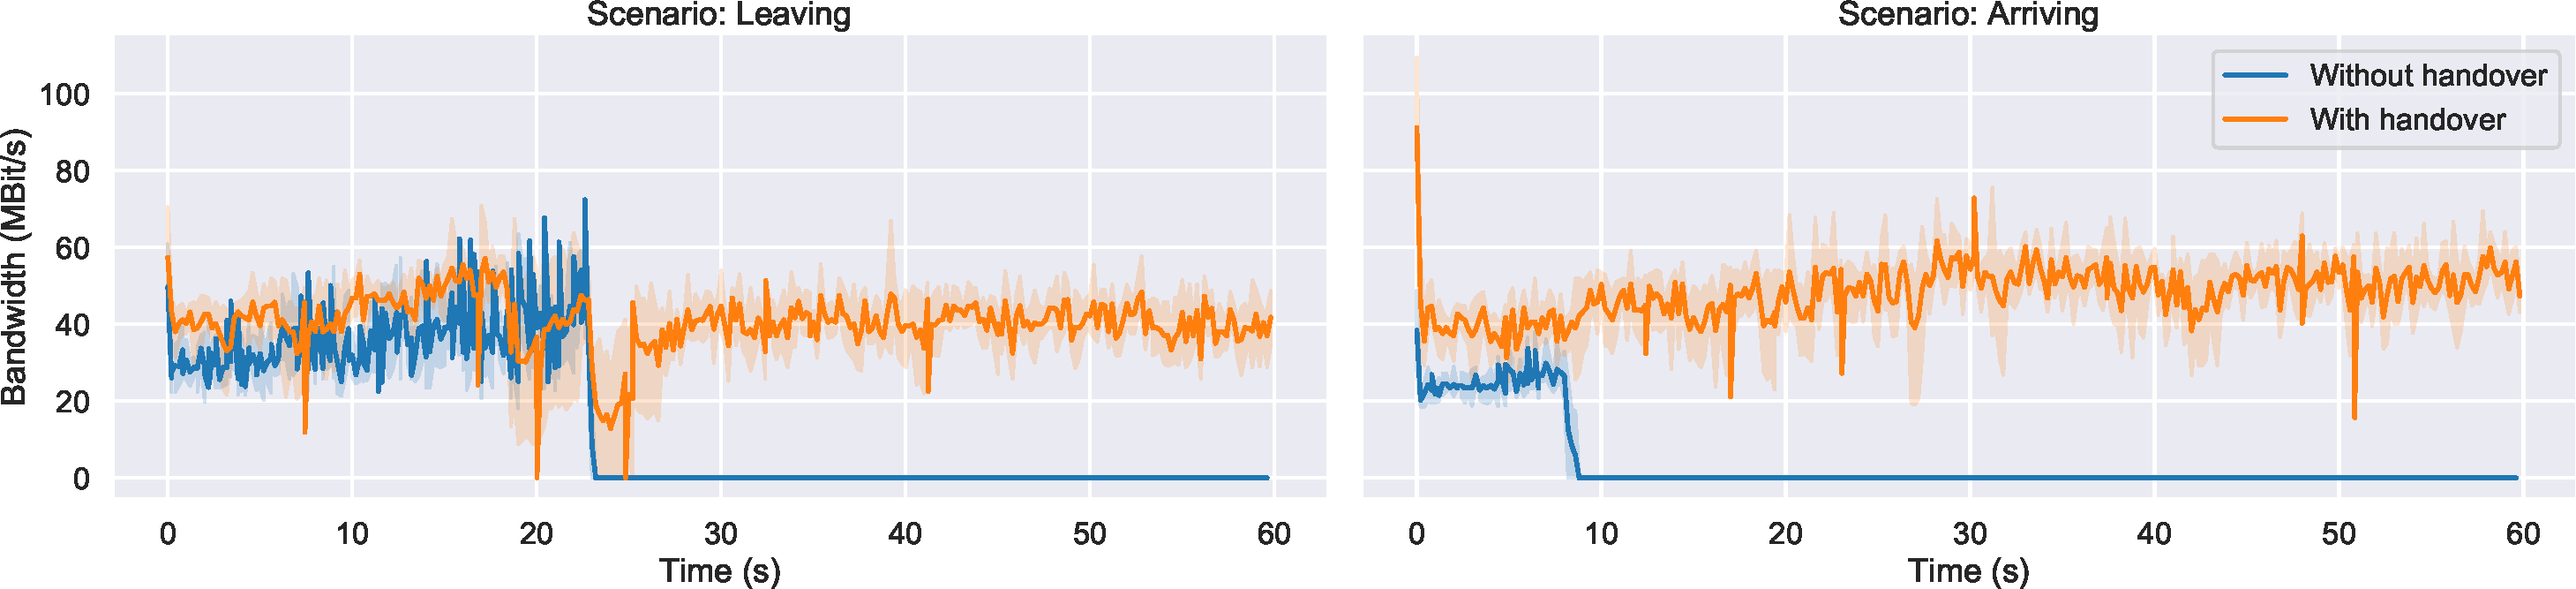
\includegraphics[width=\textwidth]{figures/migration/wg_migration-network.pdf}
    \caption{Network throughput with and without connection migration for two scenarios}
    \label{fig:eval:mig:network}
\end{figure*}
\begin{figure*}[tb]
    \centering
    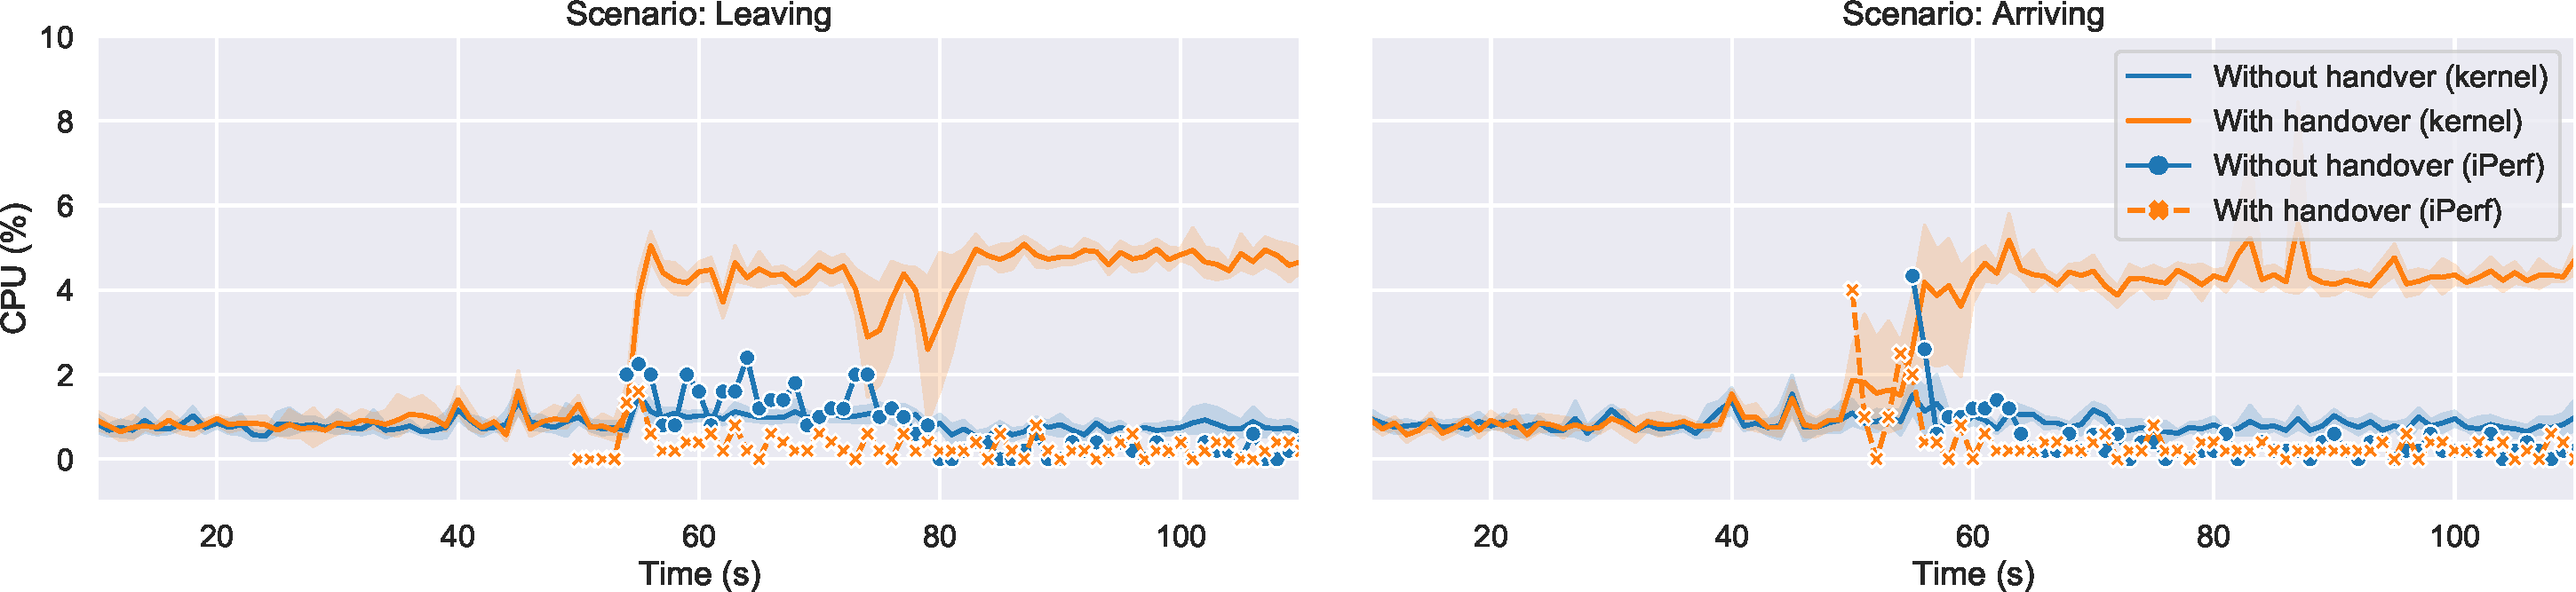
\includegraphics[width=\textwidth]{figures/migration/wg_migration-cpu.pdf}
    \caption{CPU usage with and without connection migration for two scenarios}
    \label{fig:eval:mig:cpu}
\end{figure*}


\subsubsection{Experiment Setup}
% \paragraph{Emulation}
To conduct the evaluation, two scenarios were emulated, of which the first one (S1) simulates leaving a location.
Here, the handover is performed from Wi-Fi to LTE.
The second scenario (S2) simulates the corresponding handover from LTE to Wi-Fi, e.g., when entering a building providing a Wi-Fi connection.
In order to perform these experiments, the \emph{Common Open Research Emulator (CORE)}\footnote{\url{https://coreemu.github.io}} was used, that allows execution of arbitrary programs.

\begin{figure}[ht]
    \centering
    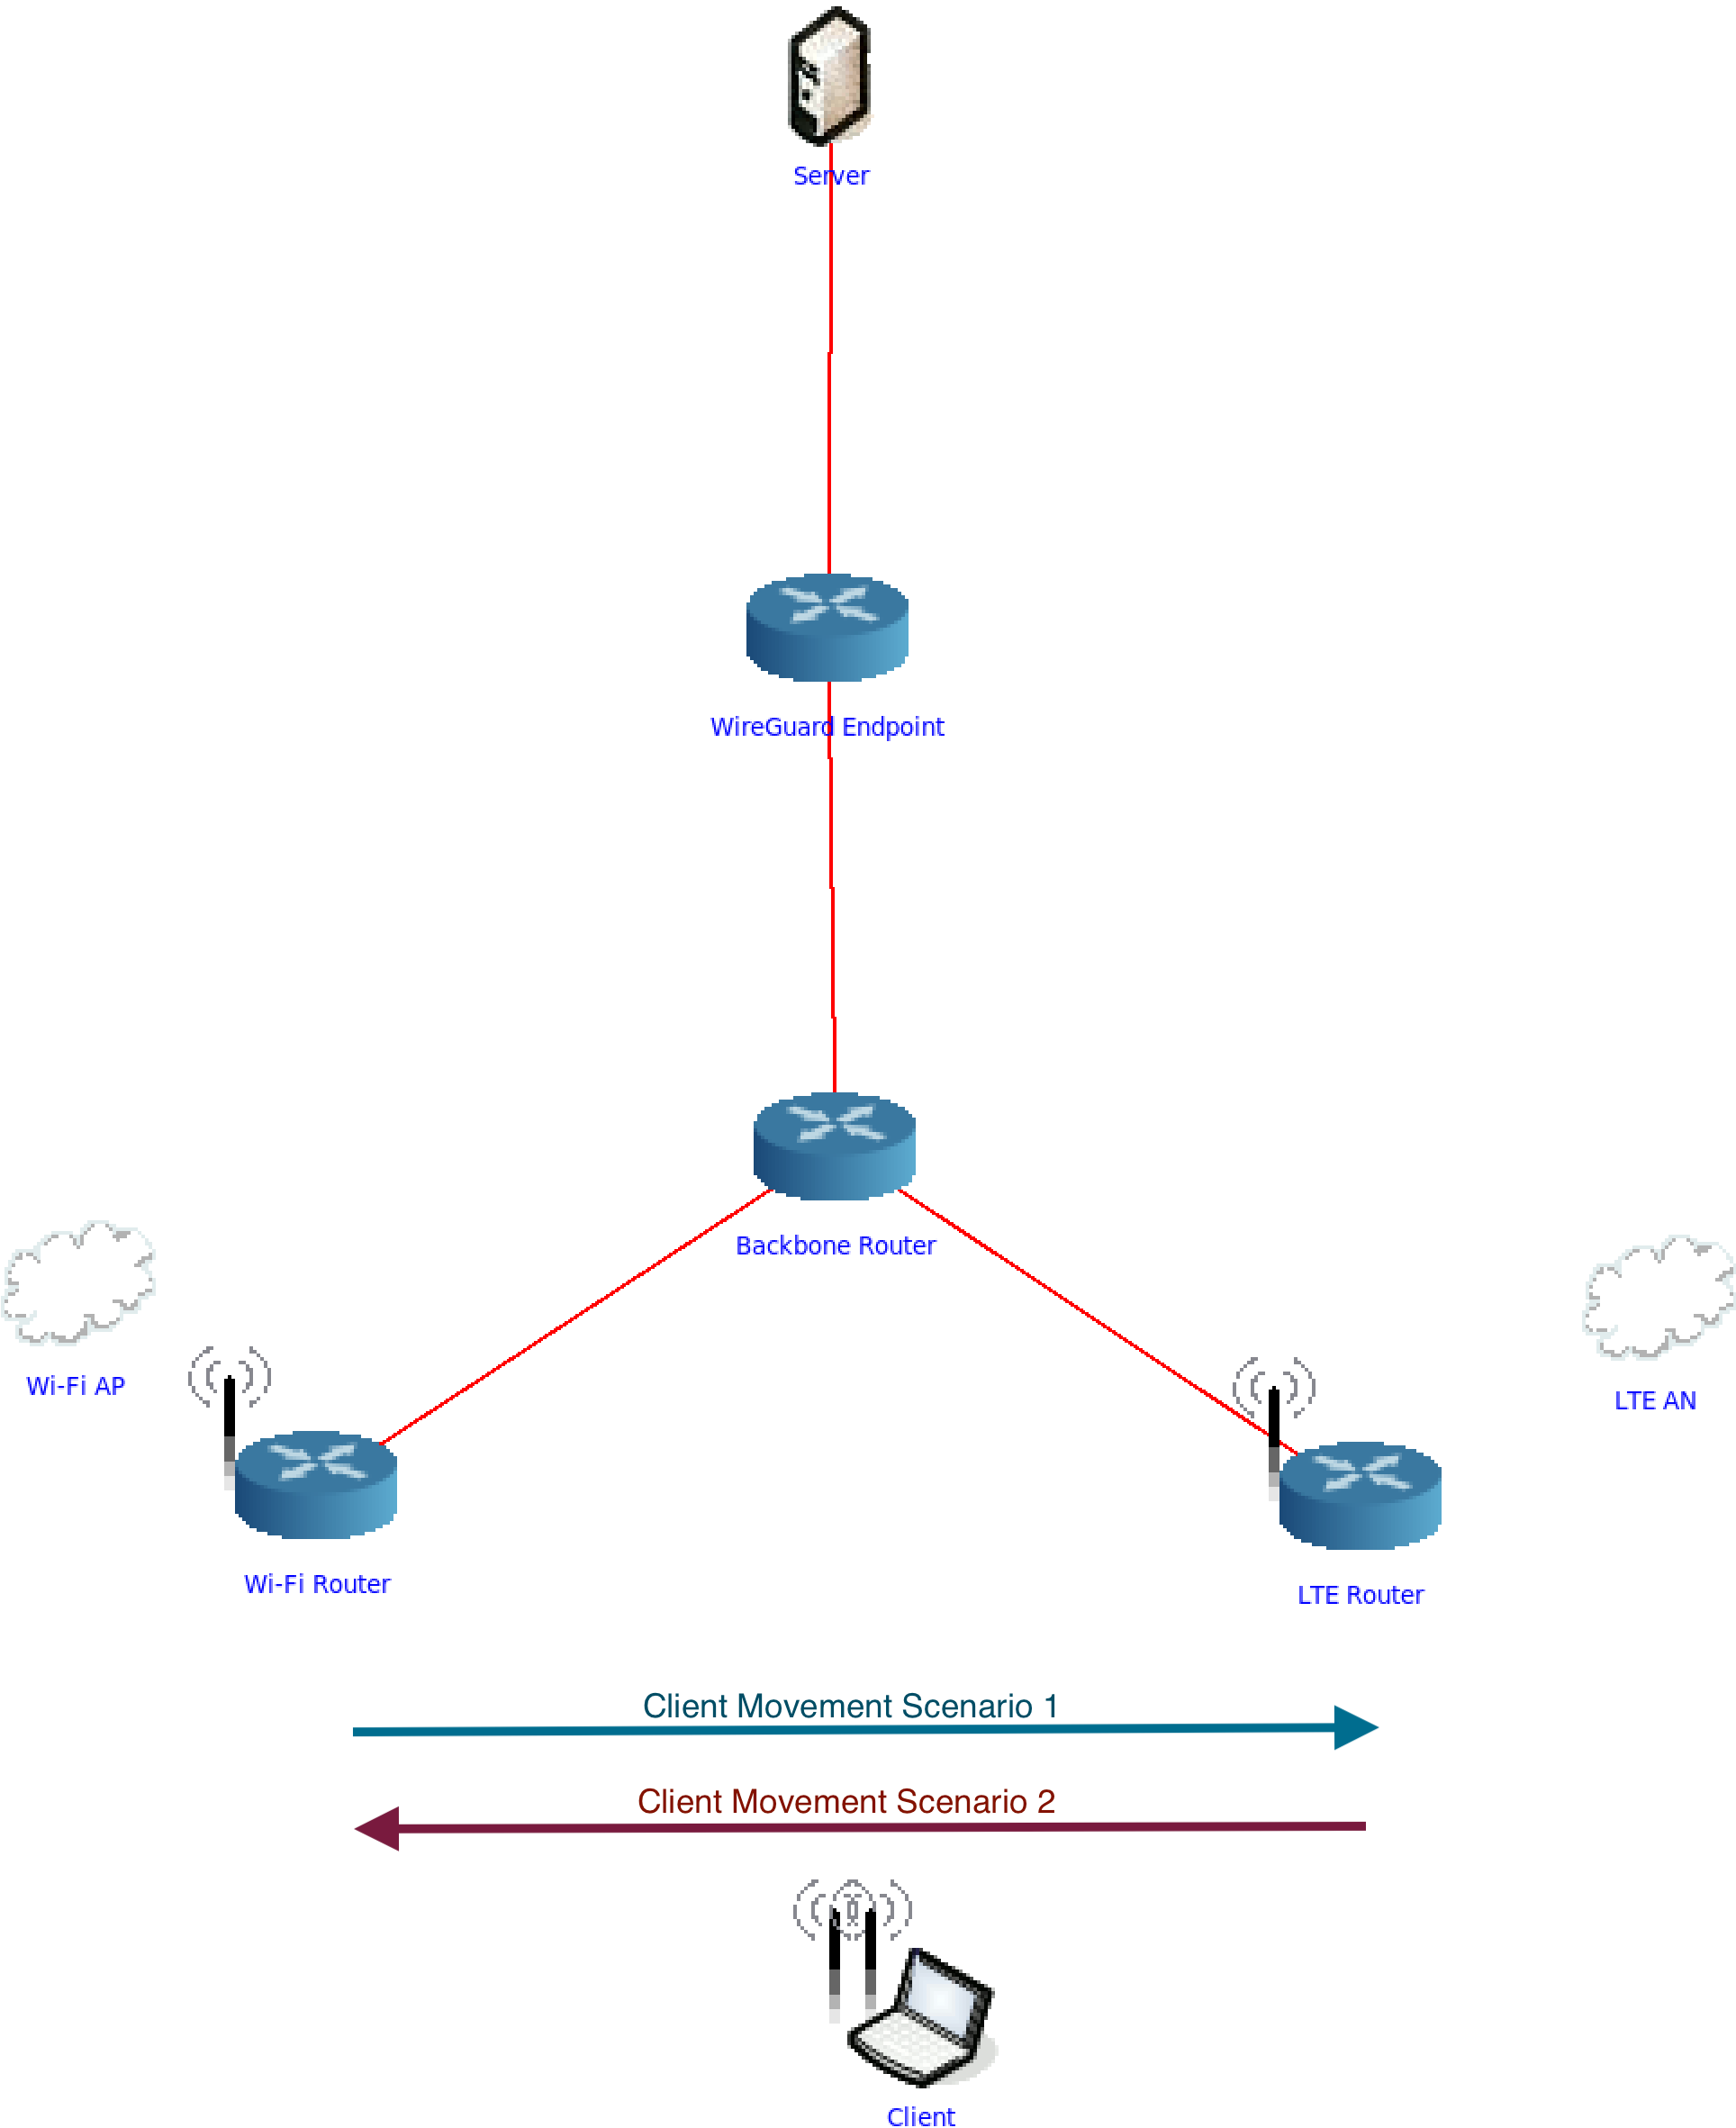
\includegraphics[width=.9\columnwidth]{figures/migration/topo.png}
    \caption{Simulated topology used for the evaluation}
    \label{fig:eval:mig:topo}
\end{figure}

% \paragraph{Topology}
Fig.~\ref{fig:eval:mig:topo} shows the topology used for the evaluation.
% Within the emulation, the following nodes were modeled.
% First, a mobile client node is required, which is the bottom node in Fig.~\ref{fig:eval:mig:topo}.
The client (bottom) contains the TCP-based application that shall be enabled with handover capabilities and the WireGuard client.
Further, the client node is the only node moving throughout the emulation.
In S1, the client moves from left to right (blue arrow) and loses the Wi-Fi connection roughly in the middle of the movement range. 
In S2, the node moves from right to left (red arrow) and regains the Wi-Fi connection at the same position.
The LTE connection is available throughout the entire experiment, whereby the Wi-Fi connection is prioritized if available.
The mobility is modeled in a way to simulate human walking, i.e., 5 to 6 km/h.
Further, we modeled a Wi-Fi access point (Wi-Fi AP on the left) and a corresponding Wi-Fi router.
% The client is connected to the Wi-Fi AP, which in turn uses the Wi-Fi router to route traffic.
We modeled the Wi-Fi AP to match the IEEE 802.11ac standard, i.e., roughly 1 Gbit/s throughput.
On the bottom right in Fig.~\ref{fig:eval:mig:topo}, the LTE access network (LTE AN) was modeled to match current LTE speeds of about 100 MBit/s.
% The LTE AN is connected to a LTE router.
In the middle of the topology, a router was modeled to mimic the backbone of the network, i.e., the network of an ISP connecting multiple parts of the Internet.
The second node from the top is the WireGuard endpoint, that is used to terminate the WireGuard tunnel.
% From this node, the arriving encapsulated TCP connection from the client is extracted and relayed to the server and TCP-packets from the server encapsulated and transmitted using WireGuard to the client.
% The WireGuard endpoint node also acts as a regular backbone router in experiments not using the WireGuard tunnel.
Finally, the server node is modeled (top), which only contains the application's server.

% The red connections in Fig.~\ref{fig:eval:mig:topo} represent wired connections between the corresponding nodes.
% The connection between the Wi-Fi router and the backbone router is modeled to mimic a standard uplink that can be found in homes with 100 MBit/s.
% The other wired connections are using links of multiple GBit/s, which are however not relevant as the limiting links are the LTE AN connection and the connection between the Wi-Fi router and backbone router.

% \paragraph{Applications}
In order to simulate a TCP-based application, iPerf3\footnote{\url{https://iperf.fr}} was used.
iPerf3 is an open-source tool for measuring network throughput in IP network following the client-server paradigm and supports various transport layer protocols.
% The server node in the evaluation topology runs an iPerf3 server, whereas the client node runs the iPerf3 client.
The client initiates the connection to the server upon experiment start using the currently active connection, i.e., Wi-Fi if available, otherwise LTE.
Each experiment was executed for 120 seconds in total.
Within the first 50 seconds, where used to allow the emulation establish routes throughout the network, so that packets can be routed from client to server and back again.
As soon as the routes were announced, the movement and iPerf started for 60 seconds.
The last 10 seconds were used to tear down the emulation.
In addition to the presented handover-approach, we also conducted experiments without a tunnel, using the regular routing mechanisms of the Linux kernel to be able to compare the achievements of our approach.
Each experiment was repeated five times to reduce effects like race conditions during booting the emulation and other side effects.

\subsubsection{Results}

% \paragraph{Supporting Vertical Handovers}
Fig.~\ref{fig:eval:mig:network} shows the results for the conducted experiments.
The x-axis denotes the experiment time, while the y-axis denotes the achieved bandwidth.
The left sub-plot visualizes the leaving scenario, while the right sub-plot visualizes the arriving scenario.
Finally, the orange graphs show experiments, where the proposed handover mechanism is enabled, the blue graphs show the results without employing the WireGuard tunnel for comparison.
As can be seen in both scenarios, the proposed approach for using WireGuard to enable TCP-based applications with vertical handover capabilities, works  as proposed.
Especially in the arriving scenario, the throughput of the iPerf application does not drop at all.
Without the WireGuard tunnel, throughput decreases because the iPerf or, in particular, the TCP connection is not re-established after the connection is changed.
In the leaving scenario, a small drop is visible at around 25 seconds.
This is due to the fact that the Wi-Fi connection is lost immediately, resulting in a short connection drop until he kernel recognizes the lost connection and propagates the changes to the routing tables.
In the arriving scenario, however, this drop is not visible since the LTE connection does not break but rather the Wi-Fi connection is established in parallel.
As soon as the kernel detects the new Wi-Fi connection, the WireGuard tunnel uses the Wi-Fi connection, whereas in the blue graph it is visible, that, although the LTE connection is still available, the TCP connection does not continue due to the newly established Wi-Fi connection.

% \paragraph{Overhead Analysis}
Although the handover capabilities offer a great improvement for users, the WireGuard tunnel introduces some kind of overhead because it has to encapsulate the TCP-connection and introduces encryption.
To quantify this overhead, the CPU usage of both the kernel and the iPerf process was monitored, which can be seen in Fig.~\ref{fig:eval:mig:cpu}.
Fig.~\ref{fig:eval:mig:cpu} is composed the same way as Fig.~\ref{fig:eval:mig:network}.
The y-axis, however, denotes the CPU utilization of the client node.
Further, the solid graphs show the kernel's CPU usage, while the graphs with markers show the CPU utilization of iPerf.
First, the iPerf CPU usage does not differ significantly, regardless of the scenario and whether the WireGuard based handover mechanism is used.
The kernel, however, shows quite a different result.
On the one hand, the blue graphs, i.e., without the WireGuard tunnel, show that the kernel's CPU utilization is relatively constant at around 1\% for the entire experiment.
In the orange graphs, on the other hand, show an increase of CPU utilization of around 3\% as soon as iPerf starts sending data, which is the same for both scenarios.
The two drops in the leaving scenario around the 80 seconds mark align with the network drop visible in Figure~\ref{fig:eval:mig:network}, where iPerf is not able to send data for the time of the handover.

Considering the improvement in the users' connection with consistently high network quality using our method, only 3\% of additional CPU consumption is an acceptable overhead.
Moreover, iPerf specifically tries to make maximum use of the available bandwidth.
For applications that have a normal usage profile, it is to expect that the overhead will be significantly lower.
Finally, the authors have shown in past work how to reliably predict Wi-Fi connection loss~\cite{hochst2019learning}.
Thus, a system that only activates the WireGuard tunnel when a connection loss is expected is conceivable, which would limit the CPU utilization overhead to a few seconds in time.
